\documentclass[12pt,final,fleqn]{article}

% basic packages
\usepackage[margin=1in] { geometry }
\usepackage{amssymb,amsmath, bm}
\usepackage{verbatim}
\usepackage[latin1]{inputenc}
%\usepackage[OT1]{fontenc}
\usepackage{setspace}
\usepackage{enumitem}
\usepackage{url}
\usepackage[font={bf}]{caption}
%\usepackage{pgfplots}
%\usepackage[font={bf}]{caption}
\usepackage{setspace}
\usepackage{latexsym}
%\usepackage{euscript}
\usepackage{graphicx}
\usepackage{marvosym}
%\usepackage[varg]{txfonts}  Older version of ``g'' in math.

% bibliography packages
\usepackage[natbibapa]{apacite}
\bibliographystyle{apsr}
\bibpunct{(}{)}{;}{a}{}{,}
\renewcommand{\bibname}{References}

% Footnote double spacing and font size for journal submission
%\usepackage{footmisc}
%\setlength{\footnotesep}{\baselineskip}
%\renewcommand{\footnotelayout}{\normalsize\doublespacing}

% hyperref options
\usepackage{color}
\usepackage{hyperref}
\usepackage{xcolor}
\hypersetup{
    colorlinks,
    linkcolor={blue!50!black},
    citecolor={blue!50!black},
    urlcolor={blue!80!black}
}
\newcommand*{\Appendixautorefname}{Appendix}
\renewcommand*{\sectionautorefname}{Section}
\renewcommand*{\subsectionautorefname}{Section}
\newcommand{\aref}[1]{\hyperref[#1]{Appendix~\ref{#1}}}

\setcounter{secnumdepth}{0}

% packages for tables
\usepackage{longtable}
\usepackage{booktabs, threeparttable}
\usepackage{threeparttablex}
%\usepackage{tabularx}
% dcolumn package
\usepackage{dcolumn}
\newcolumntype{.}{D{.}{.}{-1}}
\newcolumntype{d}[1]{D{.}{.}{#1}}
\captionsetup{belowskip=10pt,aboveskip=-5pt}
\usepackage{multirow}
% rotating package
\usepackage[figuresright]{rotating}
\usepackage{pdflscape}
\usepackage{subcaption}

% packages for figures
\usepackage{grffile}
\usepackage{afterpage}
\usepackage{float}
\usepackage[section]{placeins}
\usepackage[export]{adjustbox}

% theorem package
\usepackage{theorem}
\theoremstyle{plain}
\theoremheaderfont{\scshape}
\newtheorem{theorem}{Theorem}
\newtheorem{algorithm}{Algorithm}
\newtheorem{assumption}{Assumption}
\newtheorem{lemma}{Lemma}
\newtheorem{proposition}{Proposition}
\newtheorem{remark}{Remark}
\newcommand{\qed}{\hfill \ensuremath{\Box}}
\newcommand\indep{\protect\mathpalette{\protect\independenT}{\perp}}
\DeclareMathOperator{\sgn}{sgn}
\DeclareMathOperator{\tr}{tr}
\DeclareMathOperator{\argmin}{arg\min}
\DeclareMathOperator{\argmax}{arg\max}
\def\independenT#1#2{\mathrel{\rlap{$#1#2$}\mkern2mu{#1#2}}}
\providecommand{\norm}[1]{\lVert#1\rVert}
\renewcommand\r{\right}
\renewcommand\l{\left}
\newcommand\E{\mathbb{E}}
\newcommand\dist{\buildrel\rm d\over\sim}
\newcommand\iid{\stackrel{\rm i.i.d.}{\sim}}
\newcommand\ind{\stackrel{\rm indep.}{\sim}}
\newcommand\cov{{\rm Cov}}
\newcommand\var{{\rm Var}}
\newcommand\SD{{\rm SD}}
\newcommand\bone{\mathbf{1}}
\newcommand\bzero{\mathbf{0}}

% dotted lines in tables
%\usepackage{arydshln}

\usepackage{pdflscape}

% spacing between sections and subsections
\usepackage[compact]{titlesec}

% times new roman
%\usepackage{times}

% appendix settings
\usepackage[toc,page,header]{appendix}
\renewcommand{\appendixpagename}{\centering Appendices}
\usepackage{chngcntr}
\usepackage{etoolbox}
\usepackage{lipsum}


% file paths and definitions
\makeatletter
\newcommand*\ExpandableInput[1]{\@@input#1 }
\makeatother

\pagestyle{empty}

\setlength{\mathindent}{1cm}
\allowdisplaybreaks[4]
\doublespacing
%\special{pdf: pagesize width 8.5truein height 11.0truein}

\titleformat{\subsection}
  {\itshape\large}{\thesubsection}{1em}{}

\setcounter{tocdepth}{1}
\begin{document}
\author{Devin Incerti\thanks{Independent researcher. devin.incerti@gmail.com} and Trevor Incerti\thanks{Corresponding author. Postdoctoral Fellow, Weatherhead Center for International Affairs, Harvard University. trevorincerti@fas.harvard.edu.}}
\title{\textbf{Are regime changes always bad economics? Evidence from daily financial data \thanks{We are grateful to Peter Aronow, Matthew Graham, and Frances Rosenbluth for helpful feedback and suggestions. Authors are listed in alphabetic order, implying equal authorship. Any and all errors are our own.}}}
\date{\today}
\maketitle
\thispagestyle{empty}

\singlespacing
\begin{abstract}
\noindent
Political instability is commonly thought to discourage investment and reduce economic growth. We challenge this consensus by showing that instability does not systematically depress investment. Using an event study approach, we examine daily returns of national financial indices in every country that experienced an irregular regime change subject to data availability. Returns following resignations are large and positive (+4\%), while those following assassinations are negative and smaller in magnitude (-2\%). The impact of coups tends to be negative (-2\%), but we show that a pro-business coup results in large positive returns (+10\%). We also find evidence that authoritarian or anti-business regime changes are more likely to lead to capital flight than democratic or pro-business changes.  The immediate impact of political instability on investment is therefore dependent on the type of regime change and its expected impact on future growth. 


\end{abstract}
\doublespacing

\clearpage
\pagenumbering{arabic}

%\section{Introduction} \label{sec:Introduction}
\newpage

Economies are now global, financialized, and integrated, with domestic economies intrinsically linked to international investment. However, political instability such as coups and other regimes changes appear to jeopardize access to capital. Investors, multinational firms, development agencies, and aid organizations rank political risk as a top consideration when making investment decisions in emerging markets.\footnote{In the 2013 Multilateral Investment Guarantee Agency (MIGA) \citet{wipr2013} report (the last report published), executives of multinational enterprises (MNEs) ranked political risk as the second most important constraint for foreign direct investment (FDI) in developing countries over the next three years (after macroeconomic instability). In \citet{wipr2011} and  \citet{wipr2012}, political risk was ranked the most important constraint for FDI in developing countries - even greater than macroeconomic instability. The types of political risk of most concern to investors in developing countries (ranked in order of importance) were 1) adverse regulatory changes, 2) breaches of contract, 3) transfers and convertibility restrictions, 4) civil disturbances, 5) non-honoring of government guarantees, 6) expropriation nationalization, 7) terrorism and 8) war.} These considerations of political risk are reflected in research showing that political instability is negatively correlated with investment, financial development, and GDP growth \citep{aisen2013does, alesina1996income, alesina1996political, fosu1992political, jong2009measurement, roe2011political, baker2016measuring}, as well as associated with increases in stock market variance \citep{leblang2005government, jensen2005market, liu2015economic}. Common rationales are that unstable governments act myopically and adopt inefficient policies. Unstable governments have, for example, been argued to be less likely to invest in the legal system and the protection of property rights \citep{svensson1998investment}, and to be more likely to increases taxes \citep{devereux1998political}.\footnote{\citet{devereux1998political} proposes a model in which political instability causes governments to leave fewer assets to their successors which forces them into increasing capital taxes. The knowledge of future taxation then causes the private sector to reduce current investment which reduces future output.} 

%The image of a coup or popular uprising ousting an autocratic ruler and installing a democratic government is an evocative one. However, both recent events and prior research suggest that coups rarely lead to democracy. In the wake of the Arab Spring---in which rulers were deposed in four countries---only Tunisia ultimately transitioned to democracy. These results are in line with prior research that claims that in autocracies coups rarely lead to democratization, and in democracies they cause instability \citep{derpanopoulos2015coups, powell2011global, thyne2016coup, varol2011democratic}.



%These theories are supported by empirical research that suggests political instability---as measured by regime change frequency, political violence, or indices of uncertainty derived from news reports---is negatively correlated with investment, financial development, and GDP growth in cross country regressions \citep{aisen2013does, alesina1996income, alesina1996political, fosu1992political, jong2009measurement, roe2011political, baker2016measuring} and that the variance of stock market returns increases in response to economic policy uncertainty \citep{leblang2005government, jensen2005market, liu2015economic}.

In this study, we examine the impact of ``irregular'' regime changes and public protests on investment in a country's firms. However, unlike previous studies, we (1) remain agnostic about the direction of the effect of political instability, and (2) separately examine the effect of different types of instability on domestic firms' access to financial capital. Specifically, we examine whether changes in financial flows differ for coups, resignations, assassinations, and protests, as well as for authoritarian vs. democratic and pro vs. anti business shifts. 

%Stock market returns are used as an indicator of whether investors view different types of potentially destabilizing political events as ``good'' for future returns. 

%Beyond the large changes in real wealth created by extreme stock market volatility, empirical research has tied future production growth rates to variation in stock returns \citep{schwert1990stock, fama1990stock}.

We also provide methodological advancements when compared to the aforementioned cross country studies. Specifically, we conduct event studies of daily financial data, which estimate a local average treatment effect of an unexpected event on stock prices \textit{at the time of the event}. This interrupted time-series approach mitigates the endogeneity problems in previous cross country regressions---confounding events would need to occur on the same day as instability, and do so for a large portion of all of our independently tested events in order to influence our estimates.\footnote{A growing body of work uses event studies to assess political phenomenon.  For example, political events have been used to estimate the effect of political connections on firm value \citep[e.g.][]{fisman2001estimating,faccio2006politically,goldman2009politically}. Studies in ``forensic economics" have used abnormal returns from political events to locate or examine transactions such as insider trading \citep{dube2011coups}, illegal arms trading \citep{dellavigna2010detecting}, and the impact of hostilities on the financial performance of diamond mining firms in Angola \citep{guidolin2007diamonds}.} In addition, we integrate synthetic control and event study methods and demonstrate how ``synthetic'' control portfolios can be used to apply market-model event studies even when a suitable control portfolio is absent.

We analyze the full sample of politically unstable events for which national-level daily financial data is available---13 successful coups, 8 assassinations, 15 forced resignations, and 11 public protests.\footnote{We recognize that this does not represent a full list of historical coups, assassinations, resignations, and public protests, but are restricted to the sample of events for which national-level daily financial data is available.} We also examine the failed 2002 Venezuelan coup, as it provides a case that allows us to estimate the effects of both a seemingly successful pro-business coup, and the immediate reinstatement of a left-wing populist. Our study therefore not only uses an event-study approach to enhance the reliability of our estimates, but simultaneously examines a relatively large sample that enhances external validity and allows us to show that different types of political events have disparate effects. 

We find that coups, assassinations, resignations, and public protests cause large increases in financial volatility. However, the magnitude and direction of the effects differ by type of regime change. On average, abnormal returns following resignations are large and positive (+4\%) while abnormal returns following assassinations and coups tend to be negative and smaller in magnitude (-2\%). We also find suggestive evidence that authoritarian regime changes are more likely to lead to negative returns that democratic regime changes. Finally, we examine the effect of pro versus anti business regime change via an in-depth examination of the seemingly successful but ultimately failed coup against Hugo Chavez in 2002. Stock prices increased dramatically (+10\%) after the failed overthrow of Chavez's socialist regime and decreased by approximately the same magnitude following his return to leadership.

Our primary contributions are empirical and methodological. We provide the first estimates of the effects of different types of political instability on domestic capital access. We show that instability does not systematically depress investment, and find evidence that authoritarian regime changes are more likely to lead to negative returns, but that leaders who are clearly pro-business can be rewarded by financial markets even if they use extra-judicial methods to take power. The capital flows we document are not insubstantial---they are in some cases larger shocks than the 2008 stock market crash on their respective domestic economies. Methodologically, we (1) employ a method less susceptible to endogeneity concerns than previous studies, and (2) integrate synthetic control and event study methods to allow for control portfolios when a control candidate is not present.

\singlespacing
\section{Reexamining how markets respond to irregular regime changes}
\doublespacing

Stable capital flows are highly important to financial stability in emerging markets, which are particularly exposed to shifts in the availability of foreign capital \citep{koepke2019drives, obstfeld2012financial, cohen2017global}. High country risk reduces capital flows, which in turn has been shown to reduce domestic output growth \citep{koepke2019drives}. Conventional theory and cross-country empirical evidence suggests that political instability depresses investment \citep{irshad2017relationship, le2006political, lensink2000capital, boutchkova2012precarious, lehkonen2015democracy}. However, if market returns reflect investor expectations about future economic growth and expected returns, there are reasons to believe such hypotheses may be overly simplistic. 

First, a change in regime may be seen as a positive event if the current regime is regarded as anti-business or anti-global. Regime changes that attempt to overthrow anti-business autocrats may be expected to result in positive abnormal returns as investors see little risk of a replacement government ``worse'' than the status quo.

An active debate exists on the subject of ``good coups''---i.e. coups that lead to democratization or economic liberalization---and their effect on economic growth. \citet{alesina1996political} take the possibility of a new government adopting better economic policies seriously, but argue that the negative effects of uncertainty dominate the positive effects of coups staged by pro growth factions. \citet{alesina1996income} argue that ``unconstitional'' regime changes such as coups are worse for economic growth than other types of political instability, while \citet{londregan1990poverty} find that coups have no impact on economic growth and hypothesize that this may be because there is a bimodal distribution of coups, some of which enhance growth and others which restrict it. However, most research suggests that ``good coups'' are not the norm \citep{derpanopoulos2015coups, powell2011global, thyne2016coup, varol2011democratic}. But while ``good coups'' may be the minority, some evidence suggests that they have become more frequent \citep{marinov2014coups} and could have positive economic effects. \citet{meyersson2016political} finds that coup attempts that occur in democratic regimes are associated with negative GDP growth, while those that occur in autocratic regimes are associated with positive GDP growth. In another study examining the outcome variable as our own---financial returns---\citet{girardi2018institution} show that Salvador Allende's socialist government was associated with declines in stock prices while the coup that replaced him boosted them. 

Previous research therefore suggests that on average coups should not be expected to lead to increased economic development or positive market returns, but that positive returns associated with ``good coups'' could occasionally be present. We shed light on this theory as our event study approach also allows us to examine ``good coups''---coups that lead to democratization or economic liberalization---separately from others. As we are not limited to a single case study, we can provide both a cross-country and within-case analysis. 

Second, not all regime changes are equivalent---resignations, assassinations, and coups are all examples of sudden regime changes and have been used as proxies for instability in previous research. However, some regime changes may actually lead to increased stability. Resignations, for example, often occur when an ineffective leader steps down. Assassinations, by contrast, are not always related to the effectiveness of a leader, can occur seemingly at random, and the successor to the assassinated leader may be unclear. Coups can occur in the name of democracy or autocracy, and in general signal relative weakness in the current political system. These differences are often overlooked in past empirical strategies, which have proxied for instability in terms of the number of coups \citep{londregan1990poverty, alesina1996political}, assassinations or revolutions \citep{barro1991economic}, or have combined various metrics into single indices \citep{alesina1996income, venieris1986income, gupta1990economics}.\footnote{Note that these studies vary by metrics included in the indices, method of aggregation, and outcome variable of interest.} In another cross-country regression study, \citet{jong2009measurement} disaggregates instability into four main metrics, one of which is regime changes, but does not subset below this metric. By contrast---recognizing the different degrees of instability that these events may reflect---we estimate effects separately for coups, assassinations, resignations, and protests. Our event study approach affords us this freedom without encountering the statistical power issues that would arise in a regression setting.

Different types of regime changes may therefore have disparate effects on investment, just as they may differentially effect overall economic growth. Taken together, the theory and research above suggests that coups should on average lead to negative returns, but sometimes lead to positive returns when the coup's instigators are clearly more pro market than the regime they replace. Assassinations should have a neutral or negative impact as they increase uncertainty, but institutional responses to assassinations vary by country. By contrast, resignations may be viewed positively on average, as they typically signal the departure of an ineffective leader. 

Our empirical findings validate these predictions. We find that the type of political event and its expected impact on economic policy determines the direction of investment. Events expected to lead to more stable governance, economic liberalization, or democratization (such as willful resignations and coups that overthrow protectionist or leftist autocrats) are associated with positive returns, while those that consolidate authoritarian rule (e.g. military coups), exacerbate poor economic policies, or merely increase policy uncertainty (such as assassinations) have the opposite effect.

\section{Data}

Financial data are from the Global Financial Data database, which includes the longest available daily time series of stock prices. We collect data on national equity indices and two global equity indices, the S\&P/IFC Emerging Market Investable Composite and the Morgan Stanley Capital International (MSCI) World Index. The S\&P/IFC index includes securities from emerging markets while the MSCI index includes securities from developed markets only. We collect national stock index data on every country in which there was a coup or coup attempt, an assassination or failed assassination, or a forced resignation and for which daily financial data is available.\footnote{The list of failed assassinations are from \citet{jones2009hit}. Coup attempts are those in category 2 in the CSP Coup d'etat dataset.} The longest available daily time series for these stock indices are listed in \autoref{tab:stock-list}.

\begin{table}[!ht]
\caption{List of stock indices} \label{tab:stock-list}
\vspace{-5pt}
\footnotesize
\begin{center}
\begin{threeparttable}
\begin{tabular*}{\textwidth}{l@{\extracolsep{\fill}}lll}
  \hline
  \hline
  \multicolumn{1}{c}{Date}&\multicolumn{1}{c}{Country}&\multicolumn{1}{c}{Begin Date} &\multicolumn{1}{c}{Start Date}\\
  \hline
Argentina & Beunos Aires SE General Index & Dec-66 & Jan-17\\
Australia & Australia ASX All Ordinaries & Jan-58 & Jan-17\\
Bangladesh & Dhaka SE Index & Jan-90 & Jan-17\\
Canada & Canada S\&P/TSX 300 Composite & Jan-76 & Jan-17\\
Chile & Santiago IGBC General Index & Jan-75 & Jan-17\\
Colombia & Colombia IGBC General Index & Jan-92 & Jan-17\\
Ecuador & Ecuador Bolsa de Valores de Guayaquil (BVG) & Jan-94 & Jan-17\\
Egypt & Cairo SE Index & Dec-92 & Jan-17\\
Emerging Market & S\&P/IFC Emerging Markets Investable Composite & Jul-95 & Jan-17\\
Greece & Athens SE General Index & Oct-88 & Jan-17\\
India & Bombday SE SENSEX & Apr-79 & Jan-17\\
Indonesia & Jakarta SE Composite Index & Apr-83 & Jan-17\\
Iran & Tehran SE Price Index & Jan-95 & Jan-17\\
Israel & Tel Aviv 100 Index & May-87 & Jan-17\\
Japan & Tokyo SE Price Index (TOPIX) & Jan-53 & Jan-17\\
Latin America & Dow Jones Latin America Index & Jan-92 & Jan-17\\
Lithuania & Lithuania Lit-10 Index & Jan-99 & May-05\\
Malaysia & Malaysia KLSE Composite & Jan-80 & Jan-17\\
Nepal & Nepal NEPSE Stock Index & Jan-01 & Jan-17\\
Netherlands & Netherlands All-Share Price Index & Jan-80 & Jan-17\\
Pakistan & Karachi SE 100 Index & Jan-89 & Jan-17\\
Paraguay & Asuncion SE PDV General Index & Oct-93 & Sep-08\\
Peru & Lima SE General Index & Jan-82 & Jan-17\\
Philippines & Manila SE Composite Index & Jan-86 & Jan-17\\
Portugal & Oporto PSI-20 Index & Jan-86 & Jan-17\\
Singapore & Singapore FTSE ST Index & Jul-65 & Jan-17\\
South Korea & Korea SE Stock Price Index  & Jan-62 & Jan-17\\
Southeast Asia & Dow Jones Southeast Asia Index & Jan-92 & Jan-17\\
Spain & Madrid SE General Index & Aug-71 & Jan-17\\
Sri Lanka & Colombo SE All-Share Index & Dec-84 & Jan-17\\
Sweden & Sweden OMX Affarsvarlden General Index & Jan-80 & Jan-17\\
Taiwan & Taiwan SE Capitalization Weighted Index & Jan-67 & Jan-17\\
Thailand & Thailand SET General Index & Apr-75 & Jan-17\\
Tunisia & Tunisia SE Index & Dec-97 & Jan-17\\
Turkey & Instanbul IMKB 100 Price Index & Oct-87 & Jan-17\\
Ukraine & Ukraine PFTS OTC Index & Jan-98 & Jan-17\\
United Kingdom & UK FTSE All-Share Index & Nov-62 & Jan-17\\
United States & Dow Jones Industrial Average & Feb-1885 & Jan-17\\
Uruguay & Bolsa de Valores de Montevideo Index & Jan-08 & Jul-16\\
Venezuela & Dow Jones Venezuela Stock Index & Jan-92 & Jul-07\\
Venezuela & Caracas SE General Index & Jan-94 & Jan-17\\
World & MSCI World Price Index & Jan-76 & Jan-17\\
Zambia & Lusaka SE Index & Jan-02 & Apr-06\\
Zambia & Lusaka SE Index & Jul-11 & Jan-17\\
   \hline
   \hline
\end{tabular*}
\end{threeparttable}
\end{center}
\end{table}

Political data are primarily drawn from the Center for Systemic Peace's (CSP) Polity IV Coup d'etat dataset and Coup d'etat Events handbook. The Coup d'etat dataset includes the date of 1) successful coups, 2) attempted coups, 3) plotted coups and 4) alleged coup plots. We focus on successful coups because it is difficult to classify failed coups, and the choice of dataset and classification methodology would directly alter our findings. \citet[p. 617]{needler1966political} has gone so far as to say that ``the categories of coups that were aborted, suppressed, or abandoned melt into each other and into a host of other non-coup phenomena so as to defy accounting,'' the Center for Systemic Peace states that it is ``confident that [its] list of successful coups is comprehensive'' but does not extend this confidence to attempted or failed coups, and \citet{powell2011global} state that it is ``difficult to identify more ambiguous forms of coup activity, such as coup failures, plots, and rumors.''

\begin{table}[!ht]
\caption{Regime changes} \label{tab:regime-changes}
\vspace{-5pt}
\footnotesize
\begin{center}
\begin{threeparttable}
\begin{tabular*}{\textwidth}{l@{\extracolsep{\fill}}ll}
  \hline
  \hline
  \multicolumn{1}{c}{Date}&\multicolumn{1}{c}{Country}&\multicolumn{1}{c}{Political Outcome}\\
  \hline
   \multicolumn{3}{c}{\textbf{Coups}}\\ 
\ExpandableInput{../tables/coups.txt} \\
   \multicolumn{3}{c}{\textbf{Failed coup}}\\ 
\ExpandableInput{../tables/failed_coup.txt}\\
  \multicolumn{3}{c}{\textbf{Assassinations}}\\ 
\ExpandableInput{../tables/assassinations.txt}\\
  \multicolumn{3}{c}{\textbf{Resignations}}\\ 
\ExpandableInput{../tables/resignations.txt}
   \hline
   \hline
\end{tabular*}
\scriptsize
Notes: The Polity score is used to classify political outcomes as follows: autocracy = $-10 \leq \rm{score} \leq -6$, anocracy = $-5 \leq \rm{score} \leq 5$, and democracy = $6 \leq \rm{score} \leq 10$.
\end{threeparttable}
\end{center}
\end{table}

The Coup d'etat Events handbook also provides a list of 1) auto-coups\footnote{Defined by Center for Systemic Peace as the ``occurrence of subversion of the constitutional order by a ruling (usually elected) executive and the imposition of an autocratic regime."}, 2) the ouster of leadership by foreign forces, 3) the ouster of leadership by rebel forces, 4) assassinations of the executive and 5) resignations of the executive due to poor performance and/or loss of authority. Daily financial data is available for countries in categories 4 and 5, so we supplement the coups with assassinations and resignations to form a list of ``irregular'' regime changes. The resignations are those in which the ruling executive was coerced to resign due to poor performance, public discontent and popular demonstrations. Note that the Polity IV definition of ``poor performance'' is not synonymous with poor \textit{economic} performance, and in practice the reasons cited for resignation across events are: loss in conflict/war, anti-authoritarian protest, corruption scandals, Supreme Court ruling against unconstitutional actions, contested elections, and abuse of power. 

%loss in conflict/war (Argentina), anti-authoritarian protest (Philippines, Bangladesh, Nepal, Tunisia), corruption scandal (Philippines, Lithuania), constitutional ruling (Pakistan), contested election (Ukraine), abuse of power (Ecuador) Thailand?

We further supplement the CSP data with leadership data from Archigos Version 4.1, which allows us to identify additional cases in which a ``leader lost power through irregular means.'' Irregular transfers of power are those in which leaders do not leave office ``in a manner prescribed by either explicit rules or established conventions.'' Nearly all removals by irregular means result from the threat or use of force (e.g. coups, revolts and assassinations). 

A list of the political events in our dataset is shown in \autoref{tab:regime-changes}. Coups tend to have the largest impact on the level of democratization as a number of countries have subsequently transitioned from democracies to anocracies or autocracies. On the other hand, neither assassinations or resignations have much of an impact on the level of democratization. 

The discussion above shows that there is considerable debate about classification of regime changes. We recognize that some readers may feel that certain events are missing based on their own substantive knowledge. However, we choose to rely on commonly used third-party classifications in order to minimize the possibility that our results are driven by our own subjective classifications. The one exception is that we separately study the failed coup attempt in Venezuela in April 2002 in which the President of Venezuela, Hugo Chavez, was removed from office for two days because it provides a natural test of the impact of the seemingly successful removal of a left-wing populist with a pro-business regime, and the ensuing reinstatement of a left-wing populist. 

To gain perspective on the relationship between irregular regime changes and the stock market, \autoref{fig:AV-DR} plots the absolute value of daily stock returns averaged across all events. Returns are for 200 trading days before and after regime changes. The absolute value of returns on the event day (trading day 0) are significantly larger than on any other day. In addition, the magnitude of returns begins increasing just before the event day and remains high for a short period after. This suggests that financial volatility increases during the days surrounding regime changes, although it does not provide any evidence on mean returns.

\nameref{sec: Impact of Political Instability on Stock Returns} tests these results more formally. It will first formally estimate the amount of volatility surrounding all irregular regime changes, then analyze coups, assassinations and resignations separately and determine what impact they have on mean returns.

\begin{figure}[!ht]
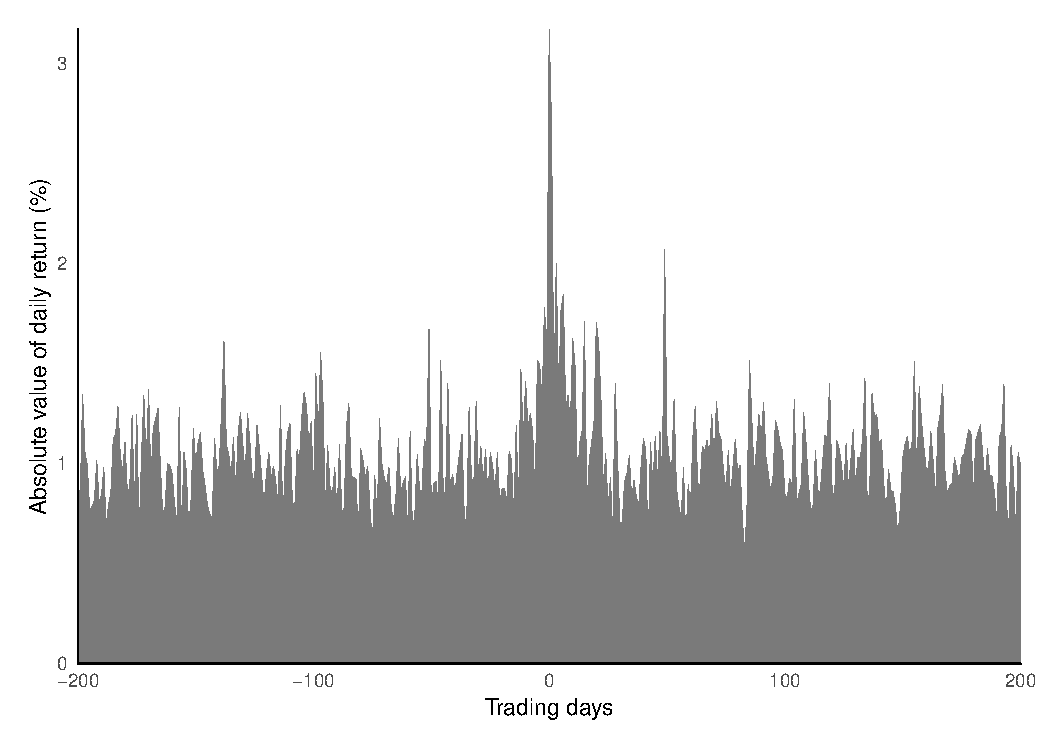
\includegraphics{../figs/daily_mean_absreturn.pdf}
\caption{Absolute value of daily returns}
\label{fig:AV-DR}
\end{figure}


\section{Impact of Political Instability on Stock Returns} \label{sec: Impact of Political Instability on Stock Returns}

\subsection{Volatility} \label{subsec: Volatility}

We first confirm that our sample of events exhibits the increases in volatility suggested by previous literature. Since stock volatility is not directly observable, one must decide how to best estimate volatility. Our estimates are obtained from a generalized autoregressive conditional heteroskedasticity (GARCH) model estimated using 1000 pre-event days, the event day and 1000 post-event days. As in \citet{jensen2005market} and \citet{leblang2005government}, we use the GARCH (1,1) specification. In particular, for national stock index $i$,
\begin{align*}
R_{it}=\mu_i + \epsilon_{it},\hspace{1cm} \epsilon_{it}\sim \mathcal{N}\left(0,\sigma_{it}^2\right),
\end{align*}
where $\mu_i$ is a constant and,
\begin{align*}
\sigma_{it}^2&=\gamma_{i}+\alpha_{i}\epsilon_{i,t-1}^2+\beta_{i}\sigma_{i,t-1}^2.
\end{align*}

The key parameter of interest is the conditional variance, $\sigma_{it}^2$. The one-period-ahead volatility forecasts, $\sigma_{it}$, are larger when $\epsilon_{i,t-1}^2$ and $\sigma_{i,t-1}^2$ are larger. In other words, the model predicts that large shocks will be followed by other large shocks.

\autoref{fig:volatility} shows the mean volatility ($\overline{\sigma_t}$) estimates from the GARCH (1,1) model across all irregular regime changes for 250 trading days prior to and 250 days after each event. As expected, the volatility estimates stay between a narrow range at nearly all dates except those surrounding the regime change. Volatility appears to increase slowly just before the regime change, albeit not to a degree out of line with previous fluctuations in volatility. This may suggest that investors sometimes have information about the events before they occur. Nonetheless, there is still an enormous volatility jump on the day of the regime change. Volatility then decreases to normal levels within a month of the event.

\begin{figure}[!htb]
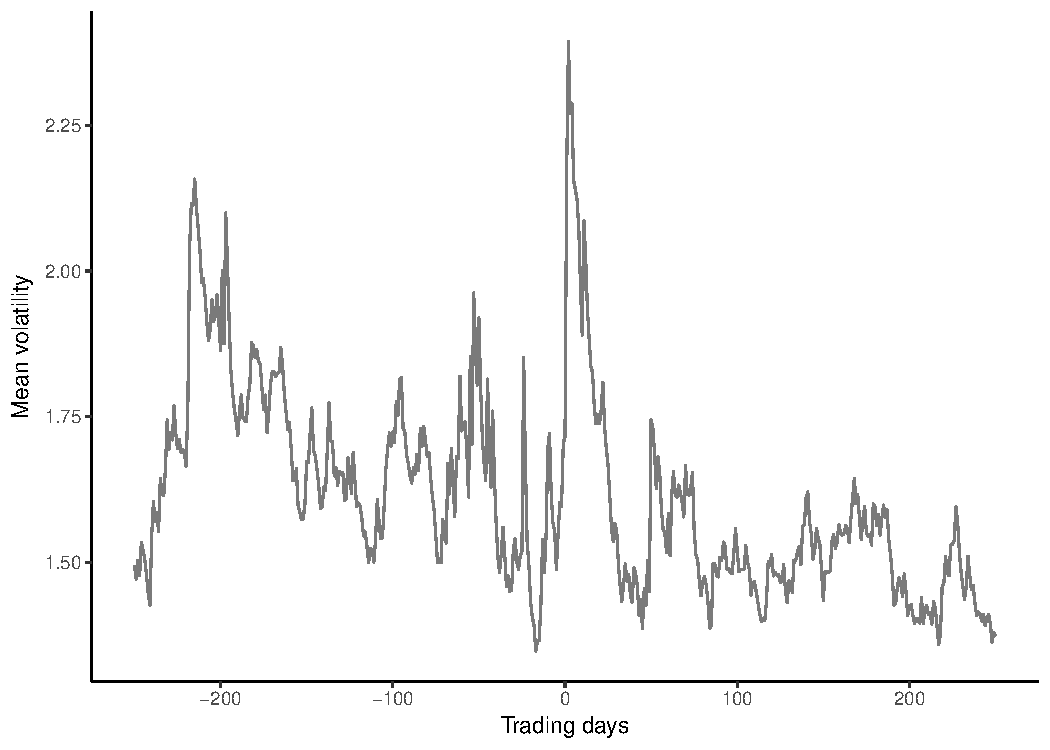
\includegraphics[scale = 0.9]{../figs/mean-volatility.pdf}
\caption{Mean of volatility estimates from GARCH(1,1) models}
\label{fig:volatility}
\end{figure}

\subsection{Abnormal Returns} \label{subsec:abnormal-returns}

We now turn to the magnitude and direction of the effect of irregular regime changes on stock returns. We follow the standard event study methodology as presented by, among others, \citet{mackinlay1997event} and \citet{campbell1997econometrics}. Normal performance is measured with a constant mean return model,
\begin{align} \label{eqn:market-model}
R_{it}=\mu_{i}+\epsilon_{it},
\end{align}
where $R_{it}$ is the logged return of national stock index $i$ on trading day $t$ and $\epsilon_{it}$ is the error term. We calculate abnormal returns (ARs), in an ``event window'' surrounding the date of each coup, $AR_{i\tau}=R_{i\tau}-\widehat{\mu}_i$, where $\tau$ is a date in the event window, and $\widehat{\mu}_i$ is estimated in an ``estimation window'' preceding the event window with \autoref{eqn:market-model}. We use a 41 day event window (i.e. 20 pre-event trading days, the event day, and 20 post-event trading days). The estimation window is the 250 trading days prior to the start of the event window. The abnormal returns are then used to generate cumulative abnormal returns (CARs) between event day $\tau_1$ and event day $\tau_2$: $CAR(\tau_1,\tau_2)=\sum_{\tau=\tau_1}^{\tau_2}AR_{i\tau}$.

A constant mean return model is used instead of a market model in order to maximize the number of observations and because our unit of analysis is country-wide market indices rather than firms.\footnote{Plausible market indices such as the MSCI World Index and the S\&P/IFC Emerging Markets Investable Composite Index only begin in 1976 and 1995, respectively.} To address concerns regarding use of a constant mean return model, we also create a synthetic control portfolio for each event and compare observed returns to the synthetic returns. 

We define the event date as the first trading day in which the market could have reacted to news of the event. For example, during the October 12, 1999 coup d'etat in Pakistan led by General Pervez Musharraf, the army announced that Prime Minister Nawaz Sharif had been dismissed after market hours at 10:15 pm. We code October 14th, the day in which the market re-opened, as the event day. When events occurred on weekends, we change the event date to the following Monday.

$(0,\tau-1)$ is used to denote the $\tau$-day period beginning with the event day and $(-1,\tau)$ to denote the negative $\tau$-day period beginning with the day prior to the event day. In other words, for cumulative abnormal returns prior to the event date, we aggregate backwards starting at the day of the event. For example, $CAR(-1,-2$) is the sum of the abnormal returns on event date $-1$ and event day $-2$. We present results for the sum of abnormal returns over the post-event windows of the event date only $(0,0$), the event date plus 6 days $(0,6$), and the event date plus 19 days $(0,19$). In addition, we present results for the pre-event windows $(-1,-7$) and $(-1,-20$).

As we hypothesize that different types of regime changes will have disparate effects on markets, we report abnormal returns separately for coups, assassinations and resignations. Standard errors and p-values are calculated using asymptotic t-statistics as in \citet{mackinlay1997event}.\footnote{It is appropriate to use the standard normal distribution to calculate test statistics because the length of the estimation window is sufficiently long (250 trading days).} 

\subsection{Coups} \label{subsec: Coups}
\autoref{tab:AR-coups} shows abnormal returns for national stock indices both preceding and following coup d'etat. \autoref{tab:AR-coups} contains all coups presented in \autoref{tab:regime-changes} with the exception of the Argentinian coup of March 24, 1976. The March 24, 1976 Argentinian coup is excluded from our analysis because the stock market remained closed from March 24 to April 5, 1976, or a period of twelve days.\footnote{Treating this twelve day period as a single day CARs results in a positive abnormal return of 58\%, a fluctuation that seems qualitatively unreasonable.} 

\begin{table}[!ht]
\caption{Abnormal returns following coups} \label{tab:AR-coups}
\vspace{-5pt}
\footnotesize
\begin{center}
\begin{threeparttable}
\begin{tabular*}{\textwidth}{l@{\extracolsep{\fill}}ld{4}d{4}d{4}d{4}d{4}d{2}}
  \hline
  \hline
\multicolumn{2}{c}{} & \multicolumn{3}{c}{Post-Event CAR} & \multicolumn{2}{c}{Pre-Event CAR} & \multicolumn{1}{c}{\multirow{2}{*}{Days to}}\\
\cmidrule(r){3-5} \cmidrule(r){6-7}
\multicolumn{1}{c}{Country} & \multicolumn{1}{c}{Event Date} & \multicolumn{1}{c}{(0,0)} & \multicolumn{1}{c}{(0,6)} & \multicolumn{1}{c}{(0,19)} & \multicolumn{1}{c}{(-1,-7)} & \multicolumn{1}{c}{(-1,-20)} & \multicolumn{1}{c}{rebound}\\
  \hline
\ExpandableInput{../tables/artable-coups-car.txt}
  \hline
\ExpandableInput{../tables/artable-coups-car-mean.txt}
   \hline
   \hline
\end{tabular*}
\scriptsize
Notes: Standard errors are in parentheses. ``Days to rebound'' is the number of trading days following a negative stock return for the national stock index to return to pre-event level (it is calculated if the price decreases on the event day, not if the event day abnormal return is negative). Returns are inflation adjusted. 
\end{threeparttable}
\end{center}
\end{table}

The average coup has a $-2.1\%$ event day AR. Event day ARs for the 1970 coup in Argentina, the 1991 coup in Thailand, the 1992 coup in Peru, and the 1999 coup in Pakistan are all negative and statistically different than zero. Moreover, all of these cases except Thailand have negative post-event CARs and pre-event CARs that are statistically indistinguishable from zero. In all of these cases, the coup either overthrew a democratically elected government or changed governance from one military ruler to another. The initial negative reaction followed by additional post-event negativity is consistent with the expected market reaction from a successful authoritarian coup followed by post-event consolidation of power. 

The only events with positive ARs are the 1971 coup in Argentina and the 2002 coup in Nepal. These results provide evidence that coups do not necessarily lead to negative abnormal returns. While the 1971 Argentinian coup did result in another military leader, it did so while calling for free and democratic elections and replaced a government that had adopted extreme protectionist economic policies. In fact, by 1973 Argentina had transitioned to a democracy.\footnote{Based on Center for System Peace Polity IV polity score of 6. Values of 6-10 are defined as democracies.} The 2002 coup in Nepal resulted in a monarchical restoration, but occurred after the country's prime minister postponed general elections, itself a democratically subversive action.  

\subsection{Assassinations} \label{subsec: Assassinations}

The results in \autoref{tab:AR-ass} are produced from analyses identical to those in \autoref{tab:AR-coups} but for successful assassinations rather than coups. Like the majority of coups, there is evidence that assassinations decrease stock prices. The mean event day abnormal return is negative and statistically different than zero. However, the result is driven by five events: the shooting of U.S. President William McKinley on September 6, 1901; the assassination of U.S. President John F. Kennedy on November 22, 1963; the assassination of Indian Prime Minister Indira Gandhi on October 31, 1984; the suicide bombing that killed Sri Lankan president Ranasinghe Premadasa on May 1, 1993; and the assassination of Israeli Prime Minister Yitzhak Rabin on the evening of November 4, 1995.

\begin{table}[!ht]
\caption{Abnormal returns following assassinations} \label{tab:AR-ass}
\vspace{-5pt}
\footnotesize
\begin{center}
\begin{threeparttable}
\begin{tabular*}{\textwidth}{l@{\extracolsep{\fill}}ld{4}d{4}d{4}d{4}d{4}d{2}}
  \hline
  \hline
\multicolumn{2}{c}{} & \multicolumn{3}{c}{Post-Event CAR} & \multicolumn{2}{c}{Pre-Event CAR} & \multicolumn{1}{c}{\multirow{2}{*}{Days to}}\\
\cmidrule(r){3-5} \cmidrule(r){6-7}
\multicolumn{1}{c}{Country} & \multicolumn{1}{c}{Event Date} & \multicolumn{1}{c}{(0,0)} & \multicolumn{1}{c}{(0,6)} & \multicolumn{1}{c}{(0,19)} & \multicolumn{1}{c}{(-1,-7)} & \multicolumn{1}{c}{(-1,-20)} & \multicolumn{1}{c}{rebound}\\
  \hline
\ExpandableInput{../tables/artable-ass-car.txt}
  \hline
\ExpandableInput{../tables/artable-ass-car-mean.txt}
   \hline
   \hline
\end{tabular*}
\scriptsize
Notes: Standard errors are in parentheses. ``Days to rebound'' is the number of trading days following a negative stock return for the national stock index to return to pre-event level (it is calculated if the price decreases on the event day, not if the event day abnormal return is negative). Returns are inflation adjusted. 
\end{threeparttable}
\end{center}
\end{table}

These results are consistent with our hypothesis that the nature of the political event and its expected impact on policy matters, and that assassinations should have a negative effect as they occur seemingly at random and increase uncertainty. While the mean effect of assassinations is negative, it is smaller in magnitude than for coups. Unlike a coup, an assassination may not necessarily be expected to cause immediate change in economic policy, particularly in the presence of an institutionalized line of succession. As such, we would expect CARs to be negative due to increased instability and uncertainty, but smaller in magnitude to a coup or resignation due to greater expectations of policy inertia.

There is no evidence of post or pre-event CARs in almost any of the assassinations. This is consistent with expectations as assassinations are typically not predictable. As with coups, the number of days that it took the stock market to rebound to pre-event levels is fairly low.\footnote{One exception is the assassination of William Mckinley in which the stock market didn't fully recover for 963 days, or almost 4 calendar years. However, this was likely caused by the Panic of 1901, which began when the stock market crashed on May 17th, 1901, and not by McKinley's death (although the assassination may have exacerbated the panic).}

\begin{table}[!ht]
\caption{Abnormal returns following resignations} \label{tab:AR-resignations}
\vspace{-5pt}
\footnotesize
\begin{center}
\begin{threeparttable}
\begin{tabular*}{\textwidth}{l@{\extracolsep{\fill}}ld{4}d{4}d{4}d{4}d{4}d{2}}
  \hline
  \hline
\multicolumn{2}{c}{} & \multicolumn{3}{c}{Post-Event CAR} & \multicolumn{2}{c}{Pre-Event CAR} & \multicolumn{1}{c}{\multirow{2}{*}{Days to}}\\
\cmidrule(r){3-5} \cmidrule(r){6-7}
\multicolumn{1}{c}{Country} & \multicolumn{1}{c}{Event Date} & \multicolumn{1}{c}{(0,0)} & \multicolumn{1}{c}{(0,6)} & \multicolumn{1}{c}{(0,19)} & \multicolumn{1}{c}{(-1,-7)} & \multicolumn{1}{c}{(-1,-20)} & \multicolumn{1}{c}{rebound}\\
  \hline
\ExpandableInput{../tables/artable-res-car.txt}
  \hline
\ExpandableInput{../tables/artable-res-car-mean.txt}
   \hline
   \hline
\end{tabular*}
\scriptsize
Notes: Standard errors are in parentheses. ``Days to rebound'' is the number of trading days following a negative stock return for the national stock index to return to pre-event level (it is calculated if the price decreases on the event day, not if the event day abnormal return is negative). Returns are inflation adjusted. 
\end{threeparttable}
\end{center}
\end{table}

\subsection{Resignations} \label{subsec: Resignations}

In contrast to coups and assassinations, abnormal returns following resignations are large and positive (see \autoref{tab:AR-resignations}). The mean event day abnormal return is over 4\% and the positive returns are persistent and grow larger over time (mean 20-day CAR $\approx$ 12\%). Furthermore, event day ARs are only negative and statistically significant at even the ten percent level in two out of the fifteen resignations (Pakistan on April 19, 1993 and Tunisia on June 31, 2011).

These results are again consistent with our hypothesis that different events will have disparate effects, and that resignations may lead to positive returns. The positive event day abnormal return following resignations is not surprising as resignations typically occur because of poor performance and/or loss of authority. Among our sample of events, leaders were ousted following loss in conflict/war, anti-authoritarian protest, corruption scandals, Supreme Court ruling against unconstitutional actions, contested elections, and abuse of power. 

For example, consider Ferdinand Marcos' resignation from office as President of the Philippines in February 1986. Prior to his resignation, the Philippine regime was known for rampant corruption, crony capitalism, extreme inequality, high unemployment, failed import substitution industrialization policy, and oligarchic control of the economy \citep{overholt1986rise, traywick2014}. In fact, the Philippines was the least preferred site for foreign investment amongst East Asian capitalist economies and possessed one of the worst capital investment to economic output ratios in Asia \citep{overholt1986rise}. Marcos held a snap presidential election on February 7, 1986, in which he declared victory despite overwhelming evidence of electoral fraud. Public protests ensued, and two weeks later the military withdrew its support of the Marcos regime \citep{lee2009armed}. Marcos was replaced by his electoral opponent, Corazon Aquino, who had run on a platform of economic liberalization and elimination of crony capitalism \citep{villegas1987philippines}. This event was associated with an approximately 13\% positive event day AR.

By contrast, the largest negative event in our sample (-3\%) is the 1993 resignation of President Ghulam Ishaq Khan and Prime Minister Nawaz Sharif in Pakistan. The resignations occurred after months of political infighting when the army demanded the President and Prime Minister resign and call for new elections. An interim prime minister was installed, but uncertainty about Pakistan's political and economic future remained high prior to the next round of elections.

The resignations studied in this paper are those in which leaders left office because of poor performance, public discontent and popular protests. It is therefore not unreasonable to expect the political actions preceding the resignations to have similarly large effects on financial markets.\footnote{Indeed, corporate investors in the 2013 MIGA \textit{World Investment and Political Risk} ranked civil disturbances as the fourth most concerning type of political risk.} To examine this, we explore all resignations that were driven by significant popular demonstrations, riots, non-violent civil resistance and other forms of public discontent in \nameref{subsec: Public Protests} in the appendix.\footnote{The set of resignations includes all those listed in either the Coup d'etat Events Handbook or the Archigos Version 4.1 data set with available financial data. In practice, this is the 2011 Egyptian Revolution and the list of resignations in \autoref{tab:AR-resignations}.} When taking directionality into account, it appears that public protests have no effect on stock returns. However, this occurs because some political movements increase stock prices while others decrease them, and the absolute value of stock returns are approximately 1.5\% higher during public protests (see \autoref{tab:protest-stocks}).\footnote{These results hold when controlling for emerging market index fluctuations.}


\section{Exploring possible mechanisms} \label{subsec: mechanisms} 

While markets may generally dislike political instability, the immediate effect of regime changes on markets may not always be unpredictable. For example, investors may generally value democracy if it is perceived to provide stronger property rights and lower susceptibility to capital appropriation \citep{przeworski1982structure, north1989constitutions, svensson1998investment}. In addition, when the successor in an irregular regime change is clear, investors may have strong priors about the effect of the new leader on economic and/or market performance. Two possible mechanisms that could be driving the differences may therefore be: (1) whether the regime change is associated with an authoritarian or democratic shift in governance, and (2) whether a new leader is clearly more pro or anti business than their predecessor. 

We first attempt to explore these mechanisms by aggregating all of the events in our sample by whether they resulted in a shift in an authoritarian or democratic direction.\footnote{As defined by the Polity project} We find suggestive evidence that regime changes associated with authoritarian shifts are on average perceived negatively by investors (see \autoref{tab:AR-auth}), while those that move governance in a democratic direction are on average perceived positively (see \autoref{tab:AR-dem}). We refer to this evidence as suggestive despite statistical significance due to the small sample of cases which fit these criteria, particularly with regard to democratic shifts. We observe ten cases associated with an authoritarian shift in governance. Only two of these events result in positive CARs, and neither are significantly different from zero. Five cases resulted in a democratic shift in governance. Three of these five cases result in positive CARs. Of the two negative CARs, one is not significantly different from zero, and the other is associated with a forced market closure that lasted 17 days. However, the majority of the positive returns from democratic regime changes come from the 12\% positive CAR associated with the resignation of Ferdinand Marcos in the Philippines in 1986. 

\begin{table}[!ht]
\caption{Abnormal returns following authoritarian regime changes} \label{tab:AR-auth}
\vspace{-5pt}
\footnotesize
\begin{center}
\begin{threeparttable}
\begin{tabular*}{\textwidth}{l@{\extracolsep{\fill}}ld{4}d{4}d{4}d{4}d{4}d{2}}
  \hline
  \hline
\multicolumn{2}{c}{} & \multicolumn{3}{c}{Post-Event CAR} & \multicolumn{2}{c}{Pre-Event CAR} & \multicolumn{1}{c}{\multirow{2}{*}{Days to}}\\
\cmidrule(r){3-5} \cmidrule(r){6-7}
\multicolumn{1}{c}{Country} & \multicolumn{1}{c}{Event Date} & \multicolumn{1}{c}{(0,0)} & \multicolumn{1}{c}{(0,6)} & \multicolumn{1}{c}{(0,19)} & \multicolumn{1}{c}{(-1,-7)} & \multicolumn{1}{c}{(-1,-20)} & \multicolumn{1}{c}{rebound}\\
  \hline
\ExpandableInput{../tables/artable-auth-car.txt}
  \hline
\ExpandableInput{../tables/artable-auth-car-mean.txt}
   \hline
   \hline
\end{tabular*}
\scriptsize
Notes: Standard errors are in parentheses. ``Days to rebound'' is the number of trading days following a negative stock return for the national stock index to return to pre-event level (it is calculated if the price decreases on the event day, not if the event day abnormal return is negative). Returns are inflation adjusted. 
\end{threeparttable}
\end{center}
\end{table}

\begin{table}[!ht]
\caption{Abnormal returns following democratic regime changes} \label{tab:AR-dem}
\vspace{-5pt}
\footnotesize
\begin{center}
\begin{threeparttable}
\begin{tabular*}{\textwidth}{l@{\extracolsep{\fill}}ld{4}d{4}d{4}d{4}d{4}d{2}}
  \hline
  \hline
\multicolumn{2}{c}{} & \multicolumn{3}{c}{Post-Event CAR} & \multicolumn{2}{c}{Pre-Event CAR} & \multicolumn{1}{c}{\multirow{2}{*}{Days to}}\\
\cmidrule(r){3-5} \cmidrule(r){6-7}
\multicolumn{1}{c}{Country} & \multicolumn{1}{c}{Event Date} & \multicolumn{1}{c}{(0,0)} & \multicolumn{1}{c}{(0,6)} & \multicolumn{1}{c}{(0,19)} & \multicolumn{1}{c}{(-1,-7)} & \multicolumn{1}{c}{(-1,-20)} & \multicolumn{1}{c}{rebound}\\
  \hline
\ExpandableInput{../tables/artable-dem-car.txt}
  \hline
\ExpandableInput{../tables/artable-dem-car-mean.txt}
   \hline
   \hline
\end{tabular*}
\scriptsize
Notes: Standard errors are in parentheses. ``Days to rebound'' is the number of trading days following a negative stock return for the national stock index to return to pre-event level (it is calculated if the price decreases on the event day, not if the event day abnormal return is negative). Returns are inflation adjusted. 
\end{threeparttable}
\end{center}
\end{table}

A similar analysis is not possible for shifts from pro or anti business leaders, as examples of such clear and plausibly exogenous shifts in leader economic ideology do not exist in our sample.\footnote{Based on matching our cases with codings from the The Ideology of Heads of Government (HOG) database, as well as surveys of news reports on the day of each event. In all cases, no clear economic ideological shift can be identified.} We therefore look outside of the sample above and conduct an in-depth case study of a seemingly pro-business and anti-socialist coup followed by the reinstatement of a socialist government: the 2002 failed coup against Hugo Chavez in Venezuela.


\begin{figure}[!ht]
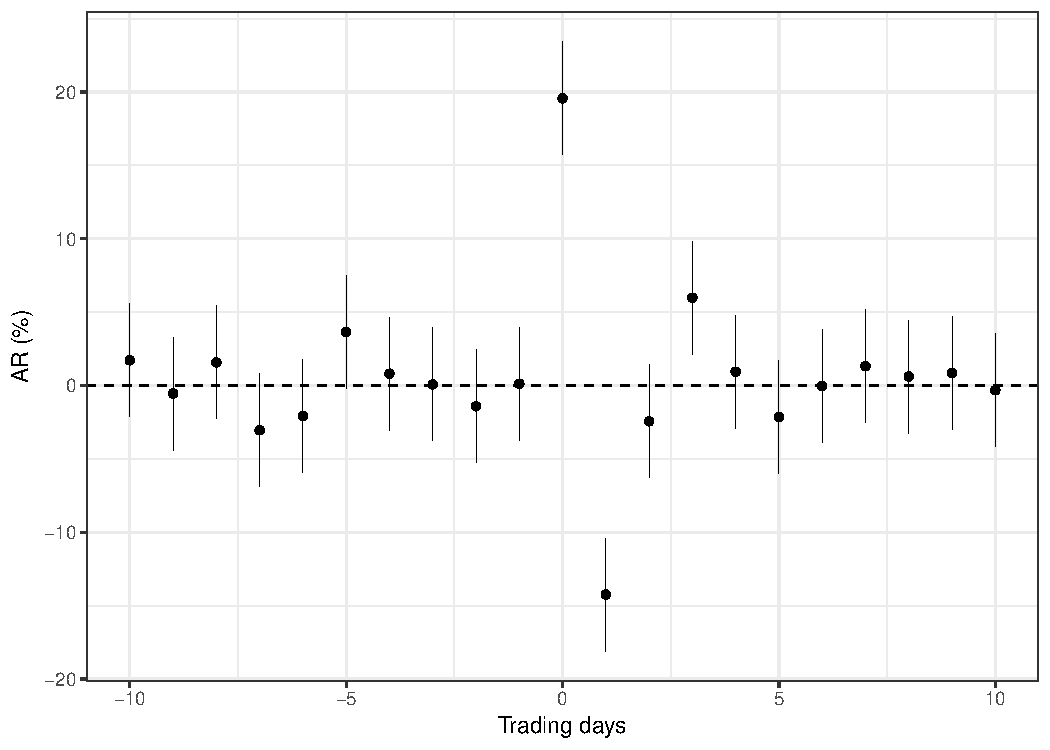
\includegraphics[width = \textwidth]{../figs/venezuela_coup_attempt_2002.pdf}
\caption{Abnormal returns surrounding the 2002 Venezuelan coup attempt}
\label{fig:AR-Ven}
\end{figure}

The ultimately failed Venezuelan coup against Hugo Chavez replaced a left-wing populist government with a new pro-business president, and therefore provides a natural test of the effects of both pro-business and anti-business regime changes separately from simple uncertainty because investors reacted to an expected regime change twice: first, when Chavez was ousted, and second, when he was reinstated. On the evening of April 11, 2002, coup plotters removed Chavez from office and later detained him. Pedro Carmona, a Venezuelan economist and business leader, was named the transitional President of Venezuela. Two days later, on April 13, 2002, a popular uprising led to Chavez's reinstatement as president. This provides an estimate of the market's valuation of a transition from the Chavez regime to the Carmona regime and its valuation of a transition from the Carmona regime back to the Chavez regime. By extension, it provides an estimate of the impact of a shift from a left-wing populist government to a pro business regime in an emerging market. 

\autoref{fig:AR-Ven} provides graphical evidence on the effect of the coup attempt. The top panel shows CARs for the 10 days prior to and following the event, along with 95\% confidence intervals. The daily ARs and corresponding confidence intervals are displayed in the bottom panel. The abnormal return on April 12, the first trading day in which investors could react to the coup, was +10\%. The market reacted in the opposite direction to Chavez's reinstatement as president: the abnormal return on the next trading day, April 15, 2002, was -8\%. 

The results in \autoref{fig:AR-Ven} are particularly striking given the discrepancy between the ARs on event days 0 and 1 and all other days. Consistent with our earlier findings that coups tend to have pre and post-event CARs that are statistically indistinguishable from zero, the only days on which the 2002 Venezuelan coup d'etat attempt ARs are statistically different from zero is on event days 0 and 1 after the coup attempt. The almost 0\% 10-day CAR preceding the coup makes this an ideal case as it implies that investors were completely unaware of the coup plot, increasing our confidence that the abnormal returns capture the true effect of the Chavez to Carmona and Carmona to Chavez regime changes on stock returns. This failed coup therefore demonstrates a large positive market reaction to the attempted overthrow of a socialist leader, and an equally large negative reaction to his reinstatement. More generally, the large magnitudes and precision of these effects suggest that  investors primarily value transition to a pro-business government regime, regardless of how the regime change is achieved. 

%We also note that Chavez's own failed attempt to overthrow the democratically elected government of Carlos Andrés Pérez---at the time pursuing deficit reduction efforts in order to obtain IMF loans---in 1992 was similarly viewed negatively by investors, resulting in an approximately -6\% AR (see \autoref{fig:AR-Ven-1992}).  Here too, pre and post-event CARs are statistically indistinguishable from zero on all days except for the day of the Chavez coup attempt, this time demonstrating the market's negative evaluation of a Pérez to Chavez regime change. These two failed coups therefore demonstrate one positive market reaction to the attempted overthrow of a socialist leader, as well as two examples of negative reactions to an attempted and successful overthrow of pro-market leaders.

\section{Robustness} \label{subsec: Robustness}

There are some potential concerns with the results in the \nameref{subsec: Coups}, \nameref{subsec: Assassinations}, and \nameref{subsec: Resignations} sections. First, the abnormal returns could have been driven by factors unrelated to the regime changes.  Second, the true effects of regime changes on firm value may be underestimated if investors had apriori information. Third, the reported means are based on small sample sizes so confidence intervals based on normally distributed abnormal returns may be inappropriate.

We explore these concerns in two ways. First, we reestimate mean CARs on a set of time-shifted placebo dates, with means computed across all events for each type of regime change. We shift event dates surrounding the actual event date backwards and forwards in increments of five days (-20, 15, 10, 5, 0, 5, 10, 15, and 20 days). In addition, we extend the forward shifted event dates to one year (110, 195, 285, and 365 days) to capture dates that are likely to be completely unaffected by the regime change. The general intuition is that we should not observe significant abnormal returns when performing an identical test on dates where no intervention (i.e. a politically unstable event) occurred. Observing such effects would call the research design and modeling assumptions into question, and raise concerns that the abnormal returns were caused by factors other than the regime changes. 

\autoref{fig:mean-car-by-regime-change} compares mean CARs estimated using the actual event date (\autoref{subfig:mean-car-by-regime-change-actual}) to CARs estimated with the event date shifted 1-year (365 days) into the future (\autoref{subfig:mean-car-by-regime-change-placebo}). \autoref{subfig:mean-car-by-regime-change-actual}---which reproduces the tabular results presented in the \nameref{subsec: Coups}, \nameref{subsec: Assassinations}, and \nameref{subsec: Resignations} sections---shows that assassinations and coups are associated with negative event day ARs while resignations are associated with positive event day ARs. In contrast, there are no discernible abnormal returns in \autoref{subfig:mean-car-by-regime-change-placebo}. The event day ARs are considerably smaller in magnitude and are not statistically different from zero for either coups or resignations. Moreover, while CARs estimated using the actual event date for resignations trend upwards following the event day, there is no consistent trend in the placebo analysis. \autoref{fig:mean-car-by-regime-change} therefore suggests that the main results are not merely an artifact of the data.  

\begin{figure}[!htb]
\centering
\begin{subfigure}{\textwidth}
\centering
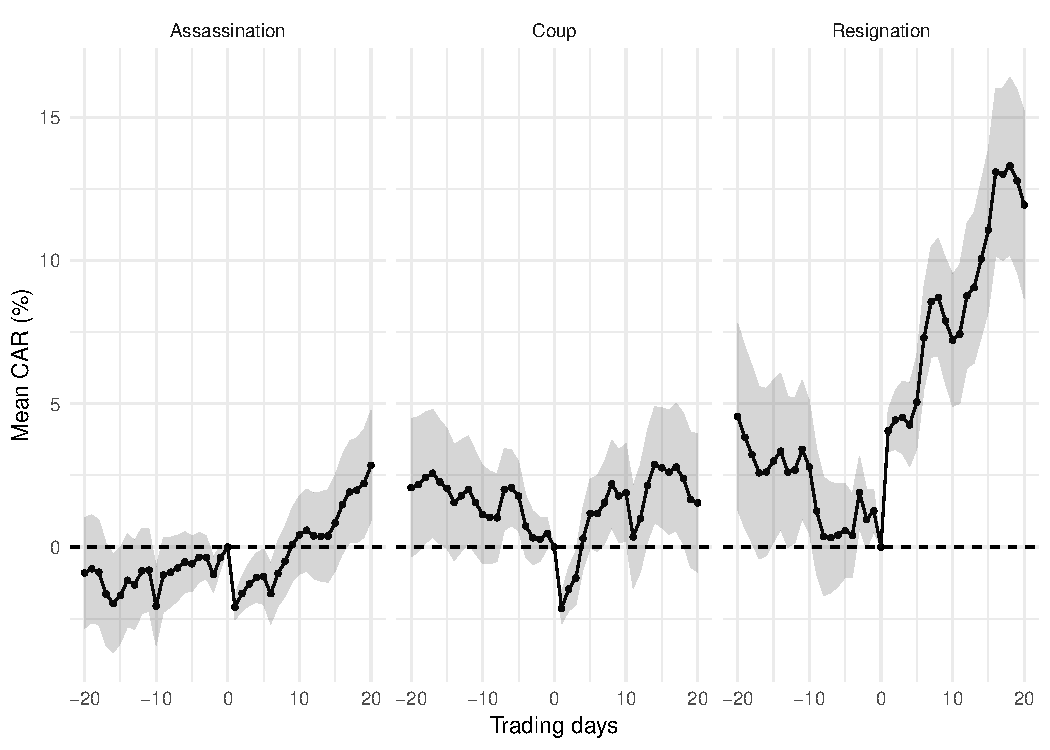
\includegraphics[max size={.8\textwidth}{.8\textheight}]{../figs/mean-car-by-regime-change-type.pdf}
\caption{Actual event date} \label{subfig:mean-car-by-regime-change-actual}
\end{subfigure}
\begin{subfigure}{\textwidth}
\centering
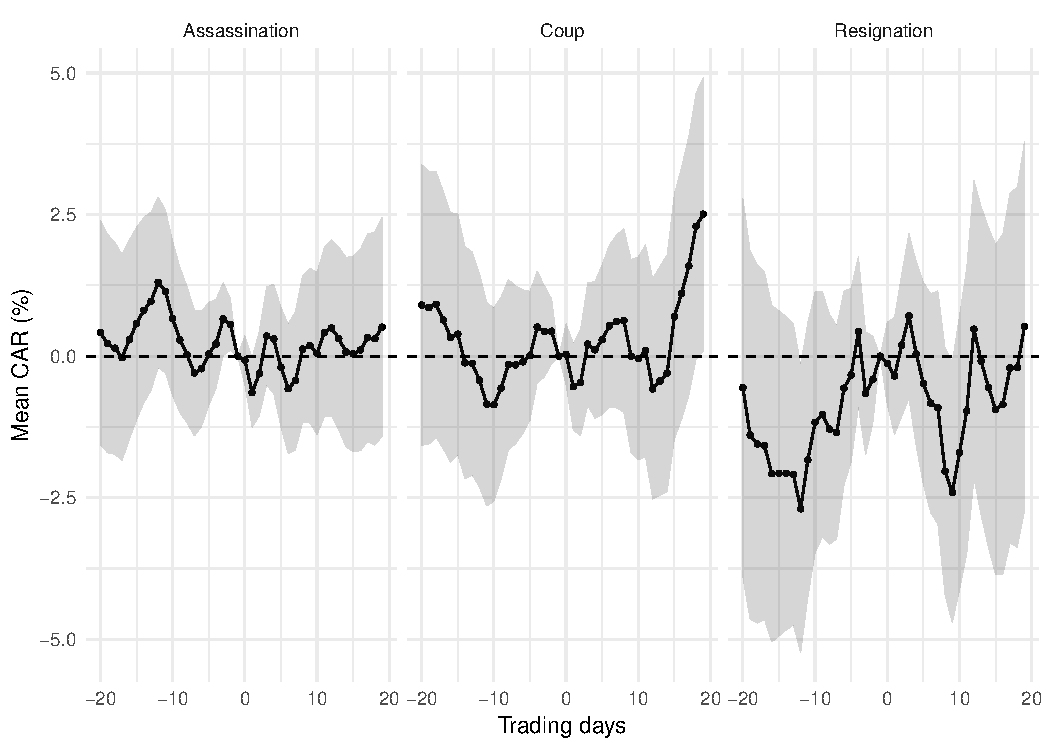
\includegraphics[max size={.8\textwidth}{.8\textheight}]{../figs/mean-car-by-regime-change-type-placebo.pdf}
\caption{Event date shifted forward by one year} \label{subfig:mean-car-by-regime-change-placebo}
\end{subfigure}
\caption{Mean cumulative abnormal returns by type of regime change}\label{fig:mean-car-by-regime-change}
\end{figure}

To ensure that results of the placebo test based on 1-year did not occur by chance, \autoref{fig:mean-event-day-ar-by-regime-change} plots event-day abnormal against the number of days shifted. There are a few instances in which there are statistically significant (at the 5\% level) ARs in the same direction as those on the actual event day, but they are always smaller in magnitude than the ARs estimated using the actual event date. Most of the statistically significant placebo estimates also occur when dates are shifted within the post-event window (days 0-20), a period during which stock returns remain volatile and, in the case of resignations, there is a consistent upward trend in the CARs. When dates are shifted forward further ($\geq$ 110 days), the event day AR is only statistically significant in one case (day 365 for assassinations). Overall, these results reinforce the main results: the ARs on the actual event date capture most of effect of the regime change, although effects can sometimes persist in the short event window following the event date. 

These figures also provide evidence on the extent to which regime changes appear to be unexpected. For instance, the CARs prior to assassinations and coups presented in \autoref{subfig:mean-car-by-regime-change-actual} tend to be close to zero, suggesting that investors were unaware that a negative event was likely to occur in the coming days. For resignations, CARs trend downward in the 10 days prior to the event; however, if investors were aware that a resignation were about to occur one would expect the pre-event CARs to be positive given the positive CARs observed in the post-event window. There is thus little evidence that the CARs in the post-event window are not capturing most of the effect caused by the regime changes.

Second, we create a synthetic control portfolio for each event based on the techniques introduced in \citet{abadie2003economic} and \citet{abadie2010synthetic}. Each country is given a weight which represents its influence in the synthetic control portfolio. The weight is chosen so that the daily returns and the variance of the daily returns of the control portfolio and the event country are most similar in the estimation window.\footnote{See ``Synthetic Control Portfolio'' in the Appendix for mathematical formalization.} The set of possible countries in the control portfolio consists of all countries listed in \autoref{tab:stock-list}.

Non-parametric statistical techniques that are free from distributional assumptions are used to address concerns about inferences from small sample sizes. We employ the sign and the rank tests, which are based on the sign and the rank of the event day ARs respectively.\footnote{See section 8 in \citet{mackinlay1997event} for more details.} Both tests are less influenced by departures from normality than statistics based on traditional t-tests such as those reported earlier in this paper. \autoref{tab:non-parametric} compares event day ARs as well as ``abnormal absolute returns'' between the event country and the synthetic control portfolio using the non-parametric methods discussed above. The ``abnormal absolute returns'' are abnormal returns for the absolute value of stock returns. This is done to combine events since resignations tend to increase returns while assassinations and coups tend to decrease them. The idea that the absolute value of returns might increase during irregular regime changes is similar to the finding that volatility increases and is consistent with \autoref{fig:AV-DR}.

\begin{table}[!ht]
\caption{Non-parametric tests of the impact of regime changes} \label{tab:non-parametric}
\vspace{-5pt}
\footnotesize
\begin{center}
\begin{threeparttable}
\begin{tabular*}{\textwidth}{l@{\extracolsep{\fill}}d{1.3}d{1.3}d{1.3}d{1.3}d{1.3}d{1.3}d{1.3}}
  \hline
  \hline
&\multicolumn{3}{c}{Regime Change Country}&\multicolumn{3}{c}{Synthetic Control Portfolio}&\multicolumn{1}{c}{\multirow{2}{*}{Wilcoxon}}\\
\cmidrule(r){2-4} \cmidrule(r){5-7}
&\multicolumn{1}{c}{Mean}&\multicolumn{1}{c}{Rank}&\multicolumn{1}{c}{Sign}
&\multicolumn{1}{c}{Mean}&\multicolumn{1}{c}{Rank}&\multicolumn{1}{c}{Sign}
&\multicolumn{1}{c}{Rank Test}\\
\multicolumn{1}{c}{Event Type}&\multicolumn{1}{c}{CAR (0,0)}&\multicolumn{1}{c}{p-value}&\multicolumn{1}{c}{p-value}
&\multicolumn{1}{c}{CAR (0,0)}&\multicolumn{1}{c}{p-value}&\multicolumn{1}{c}{p-value}
&\multicolumn{1}{c}{p-Value}\\
  \hline
\ExpandableInput{../tables/non-parametric-ar0.txt}
   \hline
   \hline
\end{tabular*}
\scriptsize
Notes: Estimates for assassinations do not include the assassination of U.S. president William McKinley in 1901 because no control portfolios are available.
\end{threeparttable}
\end{center}
\end{table}

As shown in \autoref{tab:non-parametric}, the mean event day abnormal returns for coups, assassinations and resignations are all statistically different from zero at the 1\% level using the rank test statistic and the abnormal returns for coups and assassinations are significant at at least the 10\% level using the sign test. In addition, abnormal absolute returns for all events are statistically significant at at least the 5\% level using both the rank and sign tests. On the other hand, the event day abnormal returns for the control portfolio are never statistically different from zero at even the 10\% level using the rank or sign tests. Finally, the difference in means between the regime change country and the control portfolio are statistically different from zero for coups (1\% level), assassinations (10\% level), resignations (5\% level), and all events combined (1\% level) when using two-sided p-values from the Wilcoxon rank test.\footnote{The Wilcoxon rank test is a non-parametric statistical technique that can be used to compare differences between matched samples.} In sum, the synthetic control and small sample tests suggest that the main results are not a result of deviations from normality or confounding world events.

\section{Discussion and Conclusion}

While conventional wisdom suggests investors dislike political instability, we show that this is not necessarily always the case. Unexpected changes in ruler virtually always increase market volatility, but the directionality is not always negative as markets can be given a boost when a new regime is expected to offer a more democratic or pro-business environment than the previous one. 

Coups and other types of regime changes remain common, highlighting their relevance for economic and political development. Our sample consists of 5 coups, 1 assassination, 7 resignations, and 7 instances of public protect since 2000. The Arab spring is perhaps the most notable, with protests in response to oppressive regimes and low living standards spreading throughout the Middle East in late 2010. There have also been a number of failed coups such as the 2002 coup attempt against Hugo Chavez and the 2016 failed coup in Turkey.\footnote{The Turkish coup attempt led to negative event-day CARs of approximately -7\%. See Figure A2 for a visual depiction.} Yet despite their frequency there is little evidence on their economic consequences.

This paper helps fill the evidence gap by using an event study approach that exploits daily returns of national stock market indices. This approach provides well-identified estimates of the effect of regime changes on investment that is less susceptible to endogeneity bias than prior cross country studies. Furthermore, the large sample of political events in our study increases the generalizability of our findings.  

The results are consistent with the idea that perceptions of government competence and changes in government have large impacts on investor confidence. But although the effect of regime changes and protests on stock volatility is substantial, the effect on the direction of stock returns is not uniformly negative. Abnormal returns following resignations are large and positive (+4\%), abnormal returns following assassinations are negative and smaller in magnitude (-2\%), and abnormal returns following coups also tend to be negative (-2\%). Our examination of pre-event trends in abnormal returns suggests that the positive returns we observe following resignations are not driven by investors anticipating resignations, but not coups or assassinations. CARs trend downward in the days preceding resignations, but if investors anticipated a resignation that brought a more competent leader and increased stability, pre-event CARs should also trend positive. 

A test of mechanisms suggests that democratic regime changes are typically preferable to authoritarian regime changes to investors. However, the returns surrounding the failed 2002 coup that temporarily ousted Hugo Chavez from power in Venezuela show that even democratically subversive coups can have positive effects if the instigators are clearly pro-business. These results are consistent with previous research showing that the coup replacing Allende in Chile increased stock market valuations \citep{girardi2018institution}. 

There are a number potential avenues for future research. First, more research is needed to identify the pro and anti market characteristics of regime changes. There may be pro or anti market features of regime changes that are more nuanced than those identified in this paper. Similarly, it would be useful to identify additional mechanisms through which regime changes effect investment. In the case of Chile,  \citet{girardi2018institution} show that increasing stock market valuations were caused by changes in private property rights rather than economic growth prospects or wage costs. Research focusing on the mechanisms in other settings would help generalize these findings. Lastly, it would be helpful to determine the extent to which stock market returns translate to broader economic development outcomes. \citet{meyersson2016political} has made progress on this front by examining the impact of coups on a number of outcomes in addition to economic growth including investment, debt, inflation, infant mortality, and years of schooling. It would be fruitful to examine whether the direction of the effects of different types of regime changes on these outcomes are consistent with their stock market effects, or if investor perceptions are at odds with certain development goals. Such research can help enlarge the body of evidence on the extent to which regime changes cause institutional and political change, and, in turn, have significant consequences for economic development.

\newpage


\pdfbookmark[1]{References}{References}
\bibliography{bibliography}


\newpage
\appendix
\setcounter{secnumdepth}{1}
\setcounter{table}{0}
\setcounter{figure}{0}
\renewcommand\thetable{\Alph{section}.\arabic{table}}
\renewcommand\thefigure{\Alph{section}.\arabic{figure}}

\section{Appendix} \label{sec: appendix}


\subsection{Public Protests} \label{subsec: Public Protests}

The resignations studied in this paper are those in which leaders left office because of poor performance, public discontent and popular protests. It is therefore not unreasonable to expect the political actions preceding the resignations to have similarly large effects on financial markets.\footnote{Indeed, corporate investors in the 2013 MIGA \textit{World Investment and Political Risk} ranked civil disturbances as the fourth most concerning type of political risk.} To examine this, we explore all resignations that were driven by significant popular demonstrations, riots, non-violent civil resistance and other forms of public discontent (see \autoref{tab:protest-list}).\footnote{The set of resignations includes all those listed in either the Coup d'etat Events Handbook or the Archigos Version 4.1 data set with available financial data. In practice, this is the 2011 Egyptian Revolution and the list of resignations in \autoref{tab:AR-resignations}.}

\begin{table}[!ht]
\caption{List of public protests preceding resignations} \label{tab:protest-list}
\vspace{-5pt}
\footnotesize
\begin{center}
\begin{threeparttable}
\begin{tabular*}{\textwidth}{l@{\extracolsep{\fill}}llll}
  \hline
    \hline
\multicolumn{1}{c}{Country}&\multicolumn{1}{c}{Name}&\multicolumn{1}{c}{Start Date}&\multicolumn{1}{c}{End Date}\\
  \hline
Philippines & EDSA 1/Yellow Revolution & 2/22/1986 & 2/25/1986\\
Bangladesh & Bangladeshi Spring of 1990 & 11/27/1990 & 12/7/1990\\
Thailand & Black May & 5/17/1992 & 5/20/1992\\
Indonesia & Indonesian Riots & 5/12/1998 & 5/21/1998\\
Philippines & EDSA II & 1/17/2001 & 1/20/2001\\
Argentina & Argentina Riots & 12/16/2001 & 12/20/2001\\
Ukraine & Orange Revolution & 11/22/2004 & 1/23/2005\\
Ecuador & Ecuadorian Protests & 4/13/2005 & 4/20/2005\\
Nepal & Nepalese People's Revolution & 4/6/2006 & 4/24/2006\\
Tunisia & Tunisian Revolution & 12/18/2010 & 1/14/2011\\
Egypt & Egyptian Revolution & 1/25/2011 & 2/11/2001\\
   \hline
   \hline
\end{tabular*}
\scriptsize
\end{threeparttable}
\end{center}
\end{table}

A recent example of a popular uprising preceding a resignation is the 2011 Egyptian Revolution that resulted in the overthrow of President Hosni Mubarak's regime.\footnote{Abnormal returns for this event are not shown in \autoref{tab:AR-resignations} because the stock market was closed on the day of Mubarak's resignation.} Clashes between security forces and protestors led to the deaths of hundreds of citizens and injuries to thousands more. The uprising began on January 25, 2011 when millions of protestors demanded the overthrow of the Egyptian leadership. Examples of public discontent included demonstrations, marches, riots, non-violent civil disobedience, and labor strikes.

The short-term impact of the Egyptian Revolution on the economy was disastrous. As shown in \autoref{fig:CAR-Egypt}, abnormal returns on the Egyptian Stock Exchange Index (EGX 30) were around -7\% on January 26th and -10\% the day after. To prevent further decline during the uprising, the Egyptian Stock Exchange closed at the end of trading on January 27th. President Mubarak resigned on February 11, but the market remained closed until March 23, when CARs declined by another 9\%, before rebounding slightly thereafter.

\begin{figure}[!ht]
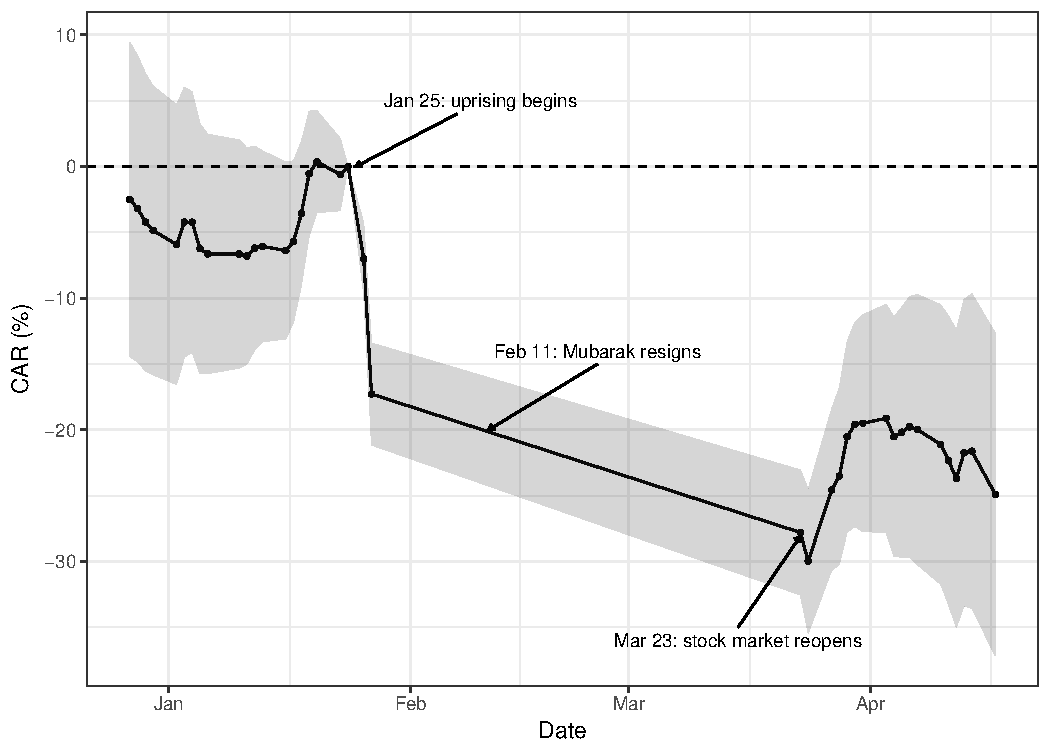
\includegraphics{../figs/egypt-revolution-2011.pdf}
\caption{Cumulative abnormal returns during the Egyptian revolution}
\label{fig:CAR-Egypt}
\end{figure}

An important question is whether other popular uprisings have had similar adverse economic consequences. To examine this, we explore all resignations that were driven by significant public protests.\footnote{The set of resignations includes all those listed in either the Coup d'etat Events Handbook or the Archigos Version 4.1 data set with available financial data. In practice, this is the 2011 Egyptian Revolution and the list or resignations in \autoref{tab:AR-resignations}.} Public protests include popular demonstrations, riots, non-violent civil resistance and other forms of public discontent. We find that both volatility and the absolute value of returns increase during times of protest. Similarly to coups, however, the direction of returns is dependent upon the nature of the protest in question. 

The start and end dates in \autoref{tab:protest-stocks} are the dates that protests began and leader's resigned respectively. Resignations caused by popular uprisings were identified by examining the descriptions in the Coup d'etat Events Handbook and Archigos Version 4.1. Additional Lexis Nexis searches were used to verify these descriptions.

In \autoref{tab:protest-stocks}, we examine whether public protests influence stock prices. The variable \textit{Protest} is equal to 1 during the dates in which citizens participate in political activities demanding the resignation of the executive and 0 otherwise. Non-protest dates are the 250 days prior to the start dates and after the end dates listed in Table A.1.\footnote{The volatility estimates used as the dependent variable in column (4) are estimated on the 250 days prior to the start date, the protest dates, and the 250 days following the end date.}

Column (1) suggests that public protests have no effect on stock returns. However, this occurs because some political movements increase stock prices while others decrease them. As shown in column (2), the absolute value of stock returns are approximately 1.5\% higher during public protests. These estimates would be biased if protest dates are correlated with higher world or regional stock market indices. To address this potential confounder, column (3) controls for returns on the S\&P/IFC Emerging Markets Investable Composite Stock Index. The coefficient on \textit{Protest} barely changes and the absolute value of returns are still about 1.5\% higher during public protests. Finally, column (4) shows that stock volatility is approximately 1 percentage point higher during political movements.\footnote{Volatility estimation methodology is described in detail in \nameref{subsec: Volatility}.}
 

We therefore find that both volatility and the absolute value of returns increase during times of protest. Similarly to coups, however, the direction of returns is dependent upon the nature of the protest in question. 

\begin{table}[!ht]
\caption{Effect of public protests on stock prices} \label{tab:protest-stocks}
\vspace{-5pt}
\footnotesize
\begin{center}
\begin{threeparttable}
\begin{tabular*}{\textwidth}{l@{\extracolsep{\fill}}d{1.3}d{1.3}d{1.3}d{1.3}}
  \hline
  \hline
\multicolumn{1}{c}{}&\multicolumn{1}{c}{Returns} & \multicolumn{2}{c}{Absolute Value of Returns}&\multicolumn{1}{c}{Volatility}\\
\cmidrule(r){2-2} \cmidrule(r){3-4} \cmidrule(r){5-5}
 & \multicolumn{1}{c}{(1)}&\multicolumn{1}{c}{(2)}&\multicolumn{1}{c}{(3)}&\multicolumn{1}{c}{(4)}\\
  \hline
\ExpandableInput{../tables/protest-regtable.txt}
   \hline
   \hline
\end{tabular*}
\scriptsize
Notes: Standard errors clustered by event are in parentheses.
\end{threeparttable}
\end{center}
\end{table}

\clearpage
\pagebreak
\newpage

\subsection{Time-shifted placebo test}

\begin{figure}[!htb]
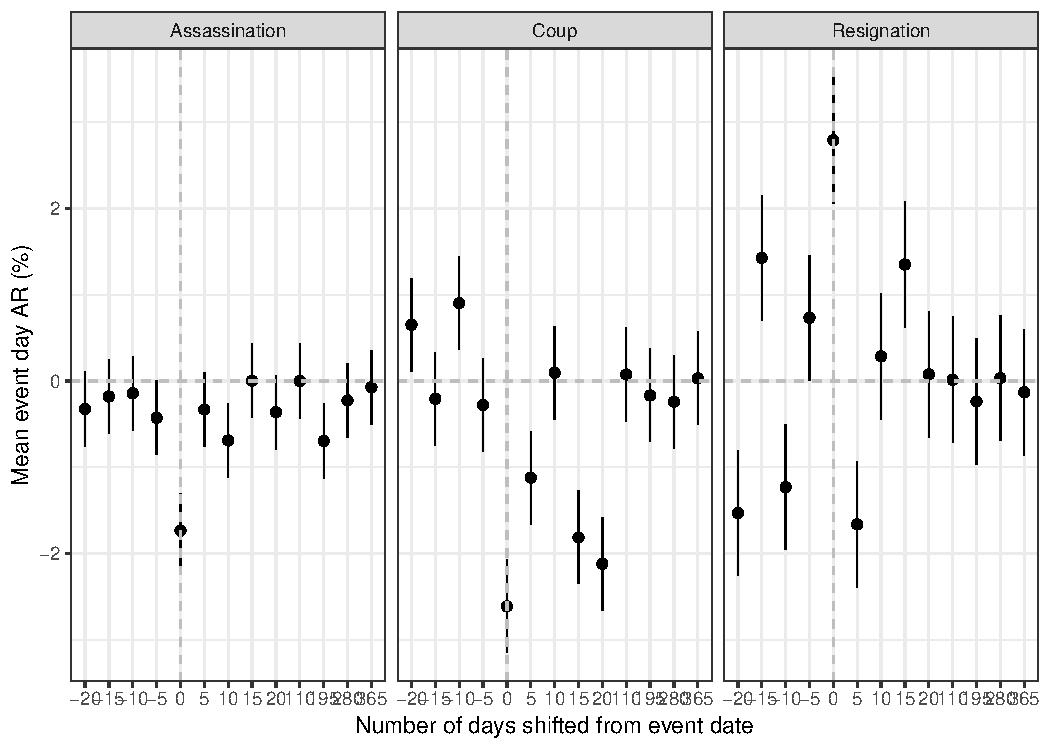
\includegraphics{../figs/mean-ar-by-regime-change-type-placebo.pdf}
\caption{Time-shifted placebo sensitivity analysis of mean event day abnormal return by type of regime change}
\label{fig:mean-event-day-ar-by-regime-change}
\end{figure}

\clearpage
\pagebreak

\subsection{Graphical depictions of additional events}

%\begin{figure}[!htb]
%\centering
%\vspace{-0.4cm}
%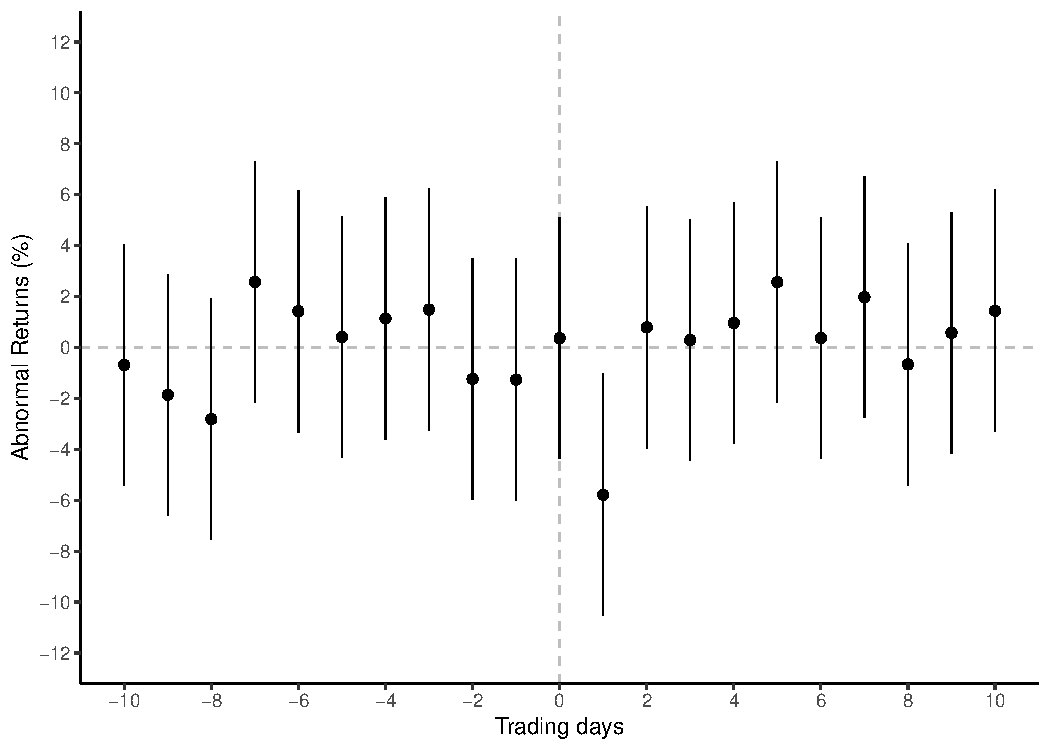
\includegraphics[scale=0.75]{../figs/venezuela_coup_attempt_1992.pdf}
%\caption{Abnormal returns surrounding the 1992 Venezuelan coup attempt}
%\label{fig:AR-Ven-1992}
%\end{figure}


\begin{figure}[!htb]
\centering
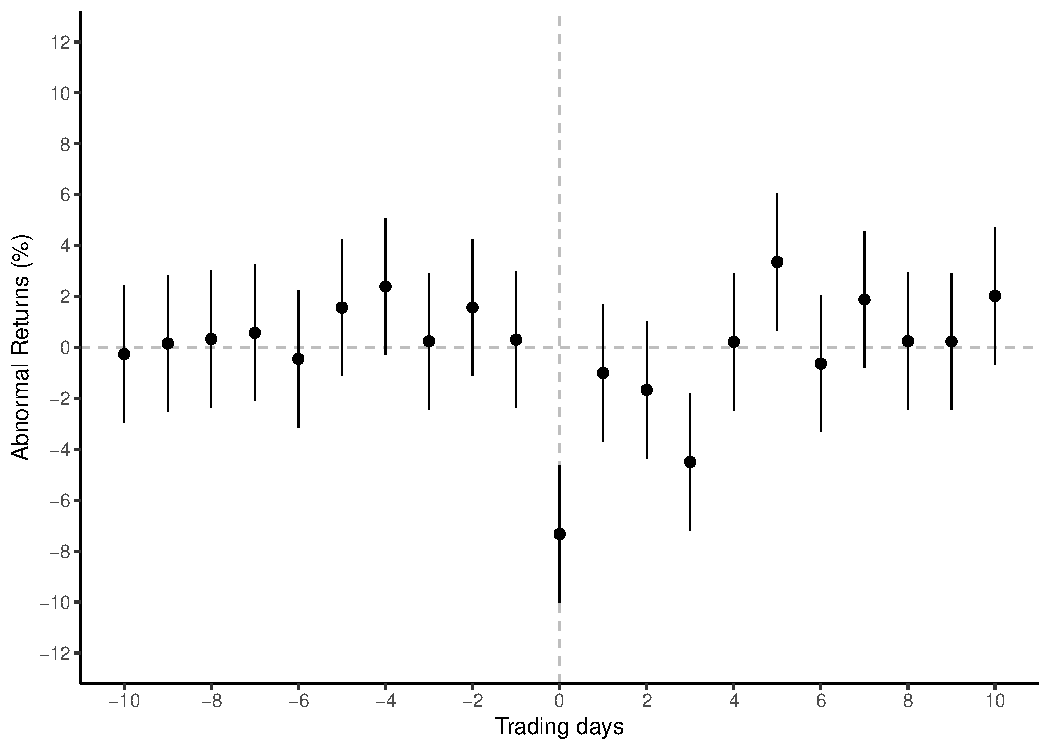
\includegraphics[scale=0.75]{../figs/turkey_coup_attempt_2016.pdf}
\caption{Abnormal returns surrounding the 2016 Turkish coup attempt}
\label{fig:AR-Turkey-2016}
\end{figure}


\pagebreak

\subsection{Synthetic Control Portfolio}\label{synthetic}
Let $\boldsymbol{R}_{k}$ be the vector of returns for the event country in the estimation window, $\boldsymbol{R}_{-k}$ be the vector of returns for all other countries in the estimation window, $\boldsymbol{X}_1=(\boldsymbol{R}_{k},\var(\boldsymbol{R}_{k}))$, $\boldsymbol{X}_0=(\boldsymbol{R}_{-k},\var(\boldsymbol{R}_{-k}))$, and $\boldsymbol{W}_{-k}$ be a $((N-1) \times 1)$ vector of weights where $N$ is the number of countries listed in \autoref{tab:stock-list}. Then $\boldsymbol{W}^*$ is chosen to minimize $(\boldsymbol{X}_1-\boldsymbol{X}_0\boldsymbol{W})'\boldsymbol{V}(\boldsymbol{X}_1-\boldsymbol{X}_0\boldsymbol{W})$ subject to $w_i\geq0$ $(i = 1,2,\ldots,N-1)$ and $\sum_i^{N-1} w_i = 1$, and the vector $\boldsymbol{V}$ is chosen so that stock returns for the control portfolio during the estimation window are are close as possible to the event country.\footnote{See \citet{abadie2003economic} for further details.}


\clearpage
\pagebreak


\end{document} 